% Options for packages loaded elsewhere
\PassOptionsToPackage{unicode}{hyperref}
\PassOptionsToPackage{hyphens}{url}
%
\documentclass[
]{article}
\usepackage{amsmath,amssymb}
\usepackage{iftex}
\ifPDFTeX
  \usepackage[T1]{fontenc}
  \usepackage[utf8]{inputenc}
  \usepackage{textcomp} % provide euro and other symbols
\else % if luatex or xetex
  \usepackage{unicode-math} % this also loads fontspec
  \defaultfontfeatures{Scale=MatchLowercase}
  \defaultfontfeatures[\rmfamily]{Ligatures=TeX,Scale=1}
\fi
\usepackage{lmodern}
\ifPDFTeX\else
  % xetex/luatex font selection
\fi
% Use upquote if available, for straight quotes in verbatim environments
\IfFileExists{upquote.sty}{\usepackage{upquote}}{}
\IfFileExists{microtype.sty}{% use microtype if available
  \usepackage[]{microtype}
  \UseMicrotypeSet[protrusion]{basicmath} % disable protrusion for tt fonts
}{}
\makeatletter
\@ifundefined{KOMAClassName}{% if non-KOMA class
  \IfFileExists{parskip.sty}{%
    \usepackage{parskip}
  }{% else
    \setlength{\parindent}{0pt}
    \setlength{\parskip}{6pt plus 2pt minus 1pt}}
}{% if KOMA class
  \KOMAoptions{parskip=half}}
\makeatother
\usepackage{xcolor}
\usepackage[margin=1in]{geometry}
\usepackage{longtable,booktabs,array}
\usepackage{calc} % for calculating minipage widths
% Correct order of tables after \paragraph or \subparagraph
\usepackage{etoolbox}
\makeatletter
\patchcmd\longtable{\par}{\if@noskipsec\mbox{}\fi\par}{}{}
\makeatother
% Allow footnotes in longtable head/foot
\IfFileExists{footnotehyper.sty}{\usepackage{footnotehyper}}{\usepackage{footnote}}
\makesavenoteenv{longtable}
\usepackage{graphicx}
\makeatletter
\def\maxwidth{\ifdim\Gin@nat@width>\linewidth\linewidth\else\Gin@nat@width\fi}
\def\maxheight{\ifdim\Gin@nat@height>\textheight\textheight\else\Gin@nat@height\fi}
\makeatother
% Scale images if necessary, so that they will not overflow the page
% margins by default, and it is still possible to overwrite the defaults
% using explicit options in \includegraphics[width, height, ...]{}
\setkeys{Gin}{width=\maxwidth,height=\maxheight,keepaspectratio}
% Set default figure placement to htbp
\makeatletter
\def\fps@figure{htbp}
\makeatother
\setlength{\emergencystretch}{3em} % prevent overfull lines
\providecommand{\tightlist}{%
  \setlength{\itemsep}{0pt}\setlength{\parskip}{0pt}}
\setcounter{secnumdepth}{-\maxdimen} % remove section numbering
\usepackage{fontspec}
\setmainfont{NanumGothic}
\ifLuaTeX
  \usepackage{selnolig}  % disable illegal ligatures
\fi
\usepackage{bookmark}
\IfFileExists{xurl.sty}{\usepackage{xurl}}{} % add URL line breaks if available
\urlstyle{same}
\hypersetup{
  pdftitle={Quiz 250310},
  pdfauthor={coop711},
  hidelinks,
  pdfcreator={LaTeX via pandoc}}

\title{Quiz 250310}
\author{coop711}
\date{2025-04-06 11:01:22}

\begin{document}
\maketitle

\section{2주차 데이터 실험
집계}\label{uxc8fcuxcc28-uxb370uxc774uxd130-uxc2e4uxd5d8-uxc9d1uxacc4}

\subsection{실험의 목적}\label{uxc2e4uxd5d8uxc758-uxbaa9uxc801}

2주차 구글 예습 설문지 집계결과를 분석합니다.

Q1\textasciitilde Q6에서는 랜덤화의 효과로 Red, Black 이 얼마나 닮았는지
알아봅니다.

Q7에서는 같은 눈속임 그래프인데 원형그래프의 각도를 속일 떄(Red)와
막대그래프의 높이를 속일 때(Black) 오류를 지각하는 데 차이가 있는지
알아봅니다.

끝으로 제출시간의 분포가 날마다 고른지, Red, Black 간에는 닮았는지
알아봅니다.

\subsubsection{Red, Black을 잘못 표시한
사람들}\label{red-blackuxc744-uxc798uxbabb-uxd45cuxc2dcuxd55c-uxc0acuxb78cuxb4e4}

\begin{longtable}[]{@{}
  >{\centering\arraybackslash}p{(\columnwidth - 6\tabcolsep) * \real{0.3056}}
  >{\centering\arraybackslash}p{(\columnwidth - 6\tabcolsep) * \real{0.1528}}
  >{\centering\arraybackslash}p{(\columnwidth - 6\tabcolsep) * \real{0.2083}}
  >{\centering\arraybackslash}p{(\columnwidth - 6\tabcolsep) * \real{0.2083}}@{}}
\toprule\noalign{}
\begin{minipage}[b]{\linewidth}\centering
제출시간
\end{minipage} & \begin{minipage}[b]{\linewidth}\centering
학번
\end{minipage} & \begin{minipage}[b]{\linewidth}\centering
랜덤화출석부
\end{minipage} & \begin{minipage}[b]{\linewidth}\centering
구글예습퀴즈
\end{minipage} \\
\midrule\noalign{}
\endhead
\bottomrule\noalign{}
\endlastfoot
2025-03-11 21:44:18 & 20223501 & Red & Black \\
2025-03-12 01:12:52 & 20246792 & Black & Red \\
2025-03-12 02:27:14 & 20242601 & Red & Black \\
2025-03-13 02:06:41 & 20246737 & Red & Black \\
2025-03-13 19:03:57 & 20241216 & Red & Black \\
2025-03-14 09:32:05 & 20241022 & Black & Red \\
2025-03-14 10:22:29 & 20231725 & Red & Black \\
2025-03-14 15:07:21 & 20243233 & Black & Red \\
2025-03-15 15:21:53 & 20213033 & Red & Black \\
2025-03-15 22:20:27 & 20241201 & Red & Black \\
2025-03-15 22:46:42 & 20243720 & Red & Black \\
2025-03-16 15:31:37 & 20223329 & Black & Red \\
2025-03-16 17:32:57 & 20211021 & Black & Red \\
2025-03-16 19:50:32 & 20241011 & Red & Black \\
2025-03-16 20:56:30 & 20213040 & Red & Black \\
2025-03-16 23:10:55 & 20241028 & Black & Red \\
2025-03-17 21:59:54 & 20242960 & Black & Red \\
2025-03-20 11:14:21 & 20246272 & Black & Red \\
2025-03-20 14:54:36 & 20246923 & Black & Red \\
2025-03-20 20:52:14 & 20242949 & Black & Red \\
2025-03-22 00:55:57 & 20246606 & Black & Red \\
2025-03-23 11:51:35 & 20242585 & Red & Black \\
2025-03-23 14:27:48 & 20243513 & Black & Red \\
2025-03-23 19:53:42 & 20227107 & Red & Black \\
\end{longtable}

\begin{longtable}[]{@{}
  >{\raggedright\arraybackslash}p{(\columnwidth - 4\tabcolsep) * \real{0.3611}}
  >{\centering\arraybackslash}p{(\columnwidth - 4\tabcolsep) * \real{0.2778}}
  >{\centering\arraybackslash}p{(\columnwidth - 4\tabcolsep) * \real{0.3056}}@{}}
\toprule\noalign{}
\begin{minipage}[b]{\linewidth}\raggedright
~
\end{minipage} & \begin{minipage}[b]{\linewidth}\centering
Red(구글예습퀴즈)
\end{minipage} & \begin{minipage}[b]{\linewidth}\centering
Black(구글예습퀴즈)
\end{minipage} \\
\midrule\noalign{}
\endhead
\bottomrule\noalign{}
\endlastfoot
\textbf{Red(랜덤화출석부)} & 268 & 12 \\
\textbf{Black(랜덤화출석부)} & 12 & 269 \\
\textbf{계} & 280 & 281 \\
\end{longtable}

랜덤화출석부에 있는 Red, Black 과 실제 구글설문에 올린 Red, Black 이
다른 사람들의 수효는 24명입니다.

Red를 Black 이라고 한 사람이 12명, Black 을 Red 라고 한 사람이
12명입니다.

두 가지 방법으로 분석합니다.

우선 Red, Black 을 잘못 선택한 24명을 랜덤하게 둘로 나누면 어느 한 쪽
집단에 들어갈 기대인원은 24명을 둘로 나눈 12(명)이고, 표준오차는 24의
제곱근에 1/2을 곱해 준 2.4명이 됩니다.

실제로 Red를 Black 이라고 한 사람수, 12명이나 Black 을 Red 라고 한
사람수, 12명은 기대인원으로부터 표준오차 범위 안에 아주 잘 들어갑니다.

두 번째 분석 방법은 확률을 계산해 보는 것입니다.

Red, Black 을 잘못 선택한 24명을 랜덤하게 둘로 나눌 때, 실제로 관찰된
12명 이상이나 12명이하로 잘못 선택한 사람수가 나올 가능성은 얼마나
되는가 입니다.

이 경우 공평한 동전던지기를 확률 법칙으로 표현한 이항분포로부터 계산할
수 있습니다.

시행횟수가 24이고 한 번 시행에서 성공확률이 1/2 인 이항분포에서
성공횟수가 12이하이거나 12이상을 관찰할 확률은 1.161입니다.

공평한 동전 던지기에서 앞면이 12개 이하 나오는 확률은 12개 이상 나오는
확률과 같기 때문에 사실상 한쪽만 계산해서 2배 해 주면 됩니다.

이 값을 p-value 라고 하는데, p-value가 0.05보다 작을 때
\textbf{통계적으로 유의한 차이를 관찰}하였다고 말합니다.

즉, 공평한 동전을 던지는 것과 같은 과정이라고 가정하였을 때 실제로
관찰된 값들이 가정으로부터 얼마나 떨어져 있는지를 표현한 것입니다.

0.05, 즉 1/20은 이런 실험을 스무 번 정도 반복하면 1번 나올 정도로 드문
사건을 의미합니다.

즉 가정이 타당하다면 나오기 힘든 결과라는 것입니다.

그런데 Red, Black 을 잘못 표시한 사람들의 분포에서 관찰된 p-value 는
0.05와는 비교도 안될 정도로 큰 값입니다.

따라서 두 집단이 랜덤화 효과가 작동하여 \textbf{통계적으로 유의한 차이를
보이지 않는다}고 할 수 있습니다.

\subsubsection{응답인원의 Red,
Black}\label{uxc751uxb2f5uxc778uxc6d0uxc758-red-black}

Red 로 응답한 인원은 280명, Black 에 응답한 인원은 281명입니다.

전체 응답인원 561 명을 랜덤하게 둘로 나눌 때 어느 한 쪽의 기대인원은
전체 응답인원의 절반인 280.5명이고, 표준오차는 전체 응답인원의 제곱근에
1/2을 곱해 준 11.8 명입니다.

따라서 Red, Black 각 그룹에 관찰된 인원은 기대인원으로부터 표준오차
범위, 혹은 두배의 표준오차 범위 안에 들어갑니다.

\subsection{Q1. 춘추전국시대에 국가통계관리의 중요성
강조}\label{q1.-uxcd98uxcd94uxc804uxad6duxc2dcuxb300uxc5d0-uxad6duxac00uxd1b5uxacc4uxad00uxb9acuxc758-uxc911uxc694uxc131-uxac15uxc870}

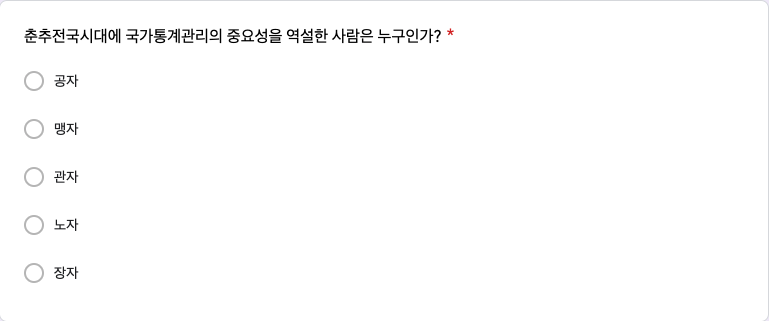
\includegraphics[width=0.75\linewidth]{./pics/Quiz210309_01}

\subsubsection{관자(집계표)}\label{uxad00uxc790uxc9d1uxacc4uxd45c}

\begin{longtable}[]{@{}
  >{\raggedright\arraybackslash}p{(\columnwidth - 12\tabcolsep) * \real{0.1667}}
  >{\centering\arraybackslash}p{(\columnwidth - 12\tabcolsep) * \real{0.0972}}
  >{\centering\arraybackslash}p{(\columnwidth - 12\tabcolsep) * \real{0.0972}}
  >{\centering\arraybackslash}p{(\columnwidth - 12\tabcolsep) * \real{0.0972}}
  >{\centering\arraybackslash}p{(\columnwidth - 12\tabcolsep) * \real{0.0972}}
  >{\centering\arraybackslash}p{(\columnwidth - 12\tabcolsep) * \real{0.0972}}
  >{\centering\arraybackslash}p{(\columnwidth - 12\tabcolsep) * \real{0.0972}}@{}}
\toprule\noalign{}
\begin{minipage}[b]{\linewidth}\raggedright
~
\end{minipage} & \begin{minipage}[b]{\linewidth}\centering
공자
\end{minipage} & \begin{minipage}[b]{\linewidth}\centering
맹자
\end{minipage} & \begin{minipage}[b]{\linewidth}\centering
관자
\end{minipage} & \begin{minipage}[b]{\linewidth}\centering
노자
\end{minipage} & \begin{minipage}[b]{\linewidth}\centering
장자
\end{minipage} & \begin{minipage}[b]{\linewidth}\centering
계
\end{minipage} \\
\midrule\noalign{}
\endhead
\bottomrule\noalign{}
\endlastfoot
\textbf{Red} & 40 & 9 & 224 & 8 & 1 & 282 \\
\textbf{Black} & 25 & 17 & 223 & 11 & 5 & 281 \\
\textbf{계} & 65 & 26 & 447 & 19 & 6 & 563 \\
\end{longtable}

\begin{longtable}[]{@{}
  >{\raggedleft\arraybackslash}p{(\columnwidth - 4\tabcolsep) * \real{0.2361}}
  >{\raggedleft\arraybackslash}p{(\columnwidth - 4\tabcolsep) * \real{0.0694}}
  >{\raggedleft\arraybackslash}p{(\columnwidth - 4\tabcolsep) * \real{0.1389}}@{}}
\caption{Pearson's Chi-squared test with simulated p-value (based on
2000 replicates): \texttt{.}}\tabularnewline
\toprule\noalign{}
\begin{minipage}[b]{\linewidth}\raggedleft
Test statistic
\end{minipage} & \begin{minipage}[b]{\linewidth}\raggedleft
df
\end{minipage} & \begin{minipage}[b]{\linewidth}\raggedleft
P value
\end{minipage} \\
\midrule\noalign{}
\endfirsthead
\toprule\noalign{}
\begin{minipage}[b]{\linewidth}\raggedleft
Test statistic
\end{minipage} & \begin{minipage}[b]{\linewidth}\raggedleft
df
\end{minipage} & \begin{minipage}[b]{\linewidth}\raggedleft
P value
\end{minipage} \\
\midrule\noalign{}
\endhead
\bottomrule\noalign{}
\endlastfoot
9.064 & NA & 0.05247 \\
\end{longtable}

Q1의 집계 결과가 Red, Black 간에 통계적으로 유의한 차이가 있는지
알아보기 위하여 카이제곱 테스트를 수행하였습니다.

그 결과 카이제곱 통계량은 9.06, 자유도는 NA , p-value 는 0.0525이므로
Red, Black 간에 통계적으로 유의한 차이를 보이지 않습니다.

실제로 닮은 게 느껴집니까?

\subsubsection{관자(\%)}\label{uxad00uxc790}

\begin{longtable}[]{@{}
  >{\centering\arraybackslash}p{(\columnwidth - 10\tabcolsep) * \real{0.0972}}
  >{\centering\arraybackslash}p{(\columnwidth - 10\tabcolsep) * \real{0.0972}}
  >{\centering\arraybackslash}p{(\columnwidth - 10\tabcolsep) * \real{0.0972}}
  >{\centering\arraybackslash}p{(\columnwidth - 10\tabcolsep) * \real{0.0972}}
  >{\centering\arraybackslash}p{(\columnwidth - 10\tabcolsep) * \real{0.0972}}
  >{\centering\arraybackslash}p{(\columnwidth - 10\tabcolsep) * \real{0.1111}}@{}}
\toprule\noalign{}
\begin{minipage}[b]{\linewidth}\centering
공자
\end{minipage} & \begin{minipage}[b]{\linewidth}\centering
맹자
\end{minipage} & \begin{minipage}[b]{\linewidth}\centering
관자
\end{minipage} & \begin{minipage}[b]{\linewidth}\centering
노자
\end{minipage} & \begin{minipage}[b]{\linewidth}\centering
장자
\end{minipage} & \begin{minipage}[b]{\linewidth}\centering
계
\end{minipage} \\
\midrule\noalign{}
\endhead
\bottomrule\noalign{}
\endlastfoot
11.5 & 4.6 & 79.4 & 3.4 & 1.1 & 100.0 \\
\end{longtable}

정답률은 Red, Black 을 합하여 계산하는데, 79.4(\%) 입니다.

\subsection{Q2. 국가정책을 수립하는 데 통계의
역할}\label{q2.-uxad6duxac00uxc815uxcc45uxc744-uxc218uxb9bduxd558uxb294-uxb370-uxd1b5uxacc4uxc758-uxc5eduxd560}

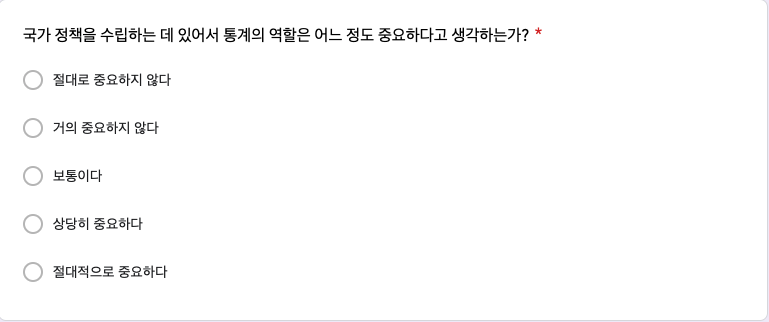
\includegraphics[width=0.75\linewidth]{./pics/Quiz210309_02}

\subsubsection{통계의
중요성(집계표)}\label{uxd1b5uxacc4uxc758-uxc911uxc694uxc131uxc9d1uxacc4uxd45c}

\begin{longtable}[]{@{}
  >{\raggedright\arraybackslash}p{(\columnwidth - 12\tabcolsep) * \real{0.1062}}
  >{\centering\arraybackslash}p{(\columnwidth - 12\tabcolsep) * \real{0.2035}}
  >{\centering\arraybackslash}p{(\columnwidth - 12\tabcolsep) * \real{0.1858}}
  >{\centering\arraybackslash}p{(\columnwidth - 12\tabcolsep) * \real{0.0973}}
  >{\centering\arraybackslash}p{(\columnwidth - 12\tabcolsep) * \real{0.1593}}
  >{\centering\arraybackslash}p{(\columnwidth - 12\tabcolsep) * \real{0.1947}}
  >{\centering\arraybackslash}p{(\columnwidth - 12\tabcolsep) * \real{0.0531}}@{}}
\toprule\noalign{}
\begin{minipage}[b]{\linewidth}\raggedright
~
\end{minipage} & \begin{minipage}[b]{\linewidth}\centering
절대로 중요하지 않다
\end{minipage} & \begin{minipage}[b]{\linewidth}\centering
거의 중요하지 않다
\end{minipage} & \begin{minipage}[b]{\linewidth}\centering
보통이다
\end{minipage} & \begin{minipage}[b]{\linewidth}\centering
상당히 중요하다
\end{minipage} & \begin{minipage}[b]{\linewidth}\centering
절대적으로 중요하다
\end{minipage} & \begin{minipage}[b]{\linewidth}\centering
계
\end{minipage} \\
\midrule\noalign{}
\endhead
\bottomrule\noalign{}
\endlastfoot
\textbf{Red} & 0 & 2 & 9 & 94 & 177 & 282 \\
\textbf{Black} & 2 & 4 & 9 & 94 & 172 & 281 \\
\textbf{계} & 2 & 6 & 18 & 188 & 349 & 563 \\
\end{longtable}

\begin{longtable}[]{@{}
  >{\raggedleft\arraybackslash}p{(\columnwidth - 4\tabcolsep) * \real{0.2361}}
  >{\raggedleft\arraybackslash}p{(\columnwidth - 4\tabcolsep) * \real{0.0694}}
  >{\raggedleft\arraybackslash}p{(\columnwidth - 4\tabcolsep) * \real{0.1389}}@{}}
\caption{Pearson's Chi-squared test with simulated p-value (based on
2000 replicates): \texttt{.}}\tabularnewline
\toprule\noalign{}
\begin{minipage}[b]{\linewidth}\raggedleft
Test statistic
\end{minipage} & \begin{minipage}[b]{\linewidth}\raggedleft
df
\end{minipage} & \begin{minipage}[b]{\linewidth}\raggedleft
P value
\end{minipage} \\
\midrule\noalign{}
\endfirsthead
\toprule\noalign{}
\begin{minipage}[b]{\linewidth}\raggedleft
Test statistic
\end{minipage} & \begin{minipage}[b]{\linewidth}\raggedleft
df
\end{minipage} & \begin{minipage}[b]{\linewidth}\raggedleft
P value
\end{minipage} \\
\midrule\noalign{}
\endhead
\bottomrule\noalign{}
\endlastfoot
2.056 & NA & 0.6472 \\
\end{longtable}

Q2의 집계 결과가 Red, Black 간에 통계적으로 유의한 차이가 있는지
알아보기 위하여 카이제곱 테스트를 수행하였습니다.

그 결과 카이제곱 통계량은 2.056, 자유도는 NA, p-value 는 0.6472이므로
Red, Black 간에 통계적으로 유의한 차이를 보이지 않습니다.

실제로 닮은 게 느껴집니까?

\subsubsection{통계의
중요성(\%)}\label{uxd1b5uxacc4uxc758-uxc911uxc694uxc131}

\begin{longtable}[]{@{}
  >{\centering\arraybackslash}p{(\columnwidth - 10\tabcolsep) * \real{0.2212}}
  >{\centering\arraybackslash}p{(\columnwidth - 10\tabcolsep) * \real{0.2019}}
  >{\centering\arraybackslash}p{(\columnwidth - 10\tabcolsep) * \real{0.1058}}
  >{\centering\arraybackslash}p{(\columnwidth - 10\tabcolsep) * \real{0.1731}}
  >{\centering\arraybackslash}p{(\columnwidth - 10\tabcolsep) * \real{0.2115}}
  >{\centering\arraybackslash}p{(\columnwidth - 10\tabcolsep) * \real{0.0865}}@{}}
\toprule\noalign{}
\begin{minipage}[b]{\linewidth}\centering
절대로 중요하지 않다
\end{minipage} & \begin{minipage}[b]{\linewidth}\centering
거의 중요하지 않다
\end{minipage} & \begin{minipage}[b]{\linewidth}\centering
보통이다
\end{minipage} & \begin{minipage}[b]{\linewidth}\centering
상당히 중요하다
\end{minipage} & \begin{minipage}[b]{\linewidth}\centering
절대적으로 중요하다
\end{minipage} & \begin{minipage}[b]{\linewidth}\centering
계
\end{minipage} \\
\midrule\noalign{}
\endhead
\bottomrule\noalign{}
\endlastfoot
0.36 & 1.07 & 3.20 & 33.39 & 61.99 & 100.00 \\
\end{longtable}

정답률은 Red, Black 을 합하여 계산하는데, 62.0(\%) 입니다.

\subsection{Q3. 우리나라 생산가능인구 감소
시기}\label{q3.-uxc6b0uxb9acuxb098uxb77c-uxc0dduxc0b0uxac00uxb2a5uxc778uxad6c-uxac10uxc18c-uxc2dcuxae30}

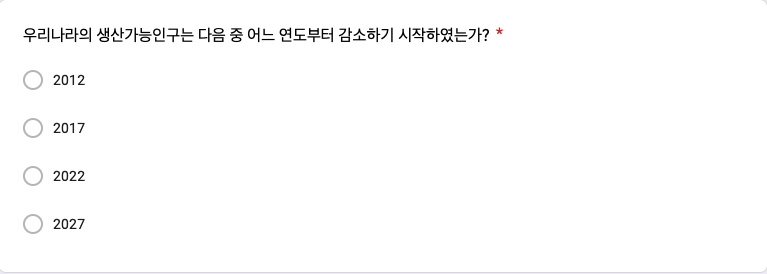
\includegraphics[width=0.75\linewidth]{./pics/Quiz210309_03}

\subsubsection{생산가능인구 감소
시기(집계표)}\label{uxc0dduxc0b0uxac00uxb2a5uxc778uxad6c-uxac10uxc18c-uxc2dcuxae30uxc9d1uxacc4uxd45c}

\begin{longtable}[]{@{}
  >{\raggedright\arraybackslash}p{(\columnwidth - 10\tabcolsep) * \real{0.1667}}
  >{\raggedleft\arraybackslash}p{(\columnwidth - 10\tabcolsep) * \real{0.0972}}
  >{\raggedleft\arraybackslash}p{(\columnwidth - 10\tabcolsep) * \real{0.0972}}
  >{\raggedleft\arraybackslash}p{(\columnwidth - 10\tabcolsep) * \real{0.0972}}
  >{\raggedleft\arraybackslash}p{(\columnwidth - 10\tabcolsep) * \real{0.0972}}
  >{\centering\arraybackslash}p{(\columnwidth - 10\tabcolsep) * \real{0.0972}}@{}}
\toprule\noalign{}
\begin{minipage}[b]{\linewidth}\raggedright
~
\end{minipage} & \begin{minipage}[b]{\linewidth}\raggedleft
2012
\end{minipage} & \begin{minipage}[b]{\linewidth}\raggedleft
2017
\end{minipage} & \begin{minipage}[b]{\linewidth}\raggedleft
2022
\end{minipage} & \begin{minipage}[b]{\linewidth}\raggedleft
2027
\end{minipage} & \begin{minipage}[b]{\linewidth}\centering
계
\end{minipage} \\
\midrule\noalign{}
\endhead
\bottomrule\noalign{}
\endlastfoot
\textbf{Red} & 31 & 224 & 23 & 4 & 282 \\
\textbf{Black} & 23 & 227 & 25 & 6 & 281 \\
\textbf{계} & 54 & 451 & 48 & 10 & 563 \\
\end{longtable}

\begin{longtable}[]{@{}
  >{\raggedleft\arraybackslash}p{(\columnwidth - 4\tabcolsep) * \real{0.2361}}
  >{\raggedleft\arraybackslash}p{(\columnwidth - 4\tabcolsep) * \real{0.0694}}
  >{\raggedleft\arraybackslash}p{(\columnwidth - 4\tabcolsep) * \real{0.1389}}@{}}
\caption{Pearson's Chi-squared test: \texttt{.}}\tabularnewline
\toprule\noalign{}
\begin{minipage}[b]{\linewidth}\raggedleft
Test statistic
\end{minipage} & \begin{minipage}[b]{\linewidth}\raggedleft
df
\end{minipage} & \begin{minipage}[b]{\linewidth}\raggedleft
P value
\end{minipage} \\
\midrule\noalign{}
\endfirsthead
\toprule\noalign{}
\begin{minipage}[b]{\linewidth}\raggedleft
Test statistic
\end{minipage} & \begin{minipage}[b]{\linewidth}\raggedleft
df
\end{minipage} & \begin{minipage}[b]{\linewidth}\raggedleft
P value
\end{minipage} \\
\midrule\noalign{}
\endhead
\bottomrule\noalign{}
\endlastfoot
1.687 & 3 & 0.6399 \\
\end{longtable}

Q3의 집계 결과가 Red, Black 간에 통계적으로 유의한 차이가 있는지
알아보기 위하여 카이제곱 테스트를 수행하였습니다.

그 결과 카이제곱 통계량은 1.687, 자유도는 3, p-value 는 0.6399이므로
Red, Black 간에 통계적으로 유의한 차이를 보이지 않습니다.

실제로 닮은 게 느껴집니까?

\subsubsection{생산가능인구 감소
시기(\%)}\label{uxc0dduxc0b0uxac00uxb2a5uxc778uxad6c-uxac10uxc18c-uxc2dcuxae30}

\begin{longtable}[]{@{}
  >{\raggedleft\arraybackslash}p{(\columnwidth - 8\tabcolsep) * \real{0.0972}}
  >{\raggedleft\arraybackslash}p{(\columnwidth - 8\tabcolsep) * \real{0.0972}}
  >{\raggedleft\arraybackslash}p{(\columnwidth - 8\tabcolsep) * \real{0.0972}}
  >{\raggedleft\arraybackslash}p{(\columnwidth - 8\tabcolsep) * \real{0.0972}}
  >{\centering\arraybackslash}p{(\columnwidth - 8\tabcolsep) * \real{0.1111}}@{}}
\toprule\noalign{}
\begin{minipage}[b]{\linewidth}\raggedleft
2012
\end{minipage} & \begin{minipage}[b]{\linewidth}\raggedleft
2017
\end{minipage} & \begin{minipage}[b]{\linewidth}\raggedleft
2022
\end{minipage} & \begin{minipage}[b]{\linewidth}\raggedleft
2027
\end{minipage} & \begin{minipage}[b]{\linewidth}\centering
계
\end{minipage} \\
\midrule\noalign{}
\endhead
\bottomrule\noalign{}
\endlastfoot
9.6 & 80.1 & 8.5 & 1.8 & 100.0 \\
\end{longtable}

정답률은 Red, Black 을 합하여 계산하는데, 80.1(\%) 입니다.

\subsection{Q4. 우리나라 총인구 최대
시기}\label{q4.-uxc6b0uxb9acuxb098uxb77c-uxcd1duxc778uxad6c-uxcd5cuxb300-uxc2dcuxae30}


\includegraphics[width=0.75\linewidth]{./pics/Quiz230308_Q4}

\subsubsection{총인구 최대
시기(집계표)}\label{uxcd1duxc778uxad6c-uxcd5cuxb300-uxc2dcuxae30uxc9d1uxacc4uxd45c}

\begin{longtable}[]{@{}
  >{\raggedright\arraybackslash}p{(\columnwidth - 10\tabcolsep) * \real{0.1667}}
  >{\raggedleft\arraybackslash}p{(\columnwidth - 10\tabcolsep) * \real{0.0972}}
  >{\raggedleft\arraybackslash}p{(\columnwidth - 10\tabcolsep) * \real{0.0972}}
  >{\raggedleft\arraybackslash}p{(\columnwidth - 10\tabcolsep) * \real{0.0972}}
  >{\raggedleft\arraybackslash}p{(\columnwidth - 10\tabcolsep) * \real{0.0972}}
  >{\centering\arraybackslash}p{(\columnwidth - 10\tabcolsep) * \real{0.0972}}@{}}
\toprule\noalign{}
\begin{minipage}[b]{\linewidth}\raggedright
~
\end{minipage} & \begin{minipage}[b]{\linewidth}\raggedleft
2018
\end{minipage} & \begin{minipage}[b]{\linewidth}\raggedleft
2019
\end{minipage} & \begin{minipage}[b]{\linewidth}\raggedleft
2020
\end{minipage} & \begin{minipage}[b]{\linewidth}\raggedleft
2021
\end{minipage} & \begin{minipage}[b]{\linewidth}\centering
계
\end{minipage} \\
\midrule\noalign{}
\endhead
\bottomrule\noalign{}
\endlastfoot
\textbf{Red} & 47 & 27 & 205 & 3 & 282 \\
\textbf{Black} & 29 & 27 & 215 & 10 & 281 \\
\textbf{계} & 76 & 54 & 420 & 13 & 563 \\
\end{longtable}

\begin{longtable}[]{@{}
  >{\raggedleft\arraybackslash}p{(\columnwidth - 4\tabcolsep) * \real{0.2361}}
  >{\raggedleft\arraybackslash}p{(\columnwidth - 4\tabcolsep) * \real{0.0694}}
  >{\raggedleft\arraybackslash}p{(\columnwidth - 4\tabcolsep) * \real{0.1667}}@{}}
\caption{Pearson's Chi-squared test with simulated p-value (based on
2000 replicates): \texttt{.}}\tabularnewline
\toprule\noalign{}
\begin{minipage}[b]{\linewidth}\raggedleft
Test statistic
\end{minipage} & \begin{minipage}[b]{\linewidth}\raggedleft
df
\end{minipage} & \begin{minipage}[b]{\linewidth}\raggedleft
P value
\end{minipage} \\
\midrule\noalign{}
\endfirsthead
\toprule\noalign{}
\begin{minipage}[b]{\linewidth}\raggedleft
Test statistic
\end{minipage} & \begin{minipage}[b]{\linewidth}\raggedleft
df
\end{minipage} & \begin{minipage}[b]{\linewidth}\raggedleft
P value
\end{minipage} \\
\midrule\noalign{}
\endhead
\bottomrule\noalign{}
\endlastfoot
8.269 & NA & 0.03198 * \\
\end{longtable}

Q4의 집계 결과가 Red, Black 간에 통계적으로 유의한 차이가 있는지
알아보기 위하여 카이제곱 테스트를 수행하였습니다.

그 결과 카이제곱 통계량은 8.269, 자유도는 NA, p-value 는 0.0320이므로
Red, Black 간에 통계적으로 유의한 차이를 보이고 있습니다.

\subsubsection{총인구 최대
시기(\%)}\label{uxcd1duxc778uxad6c-uxcd5cuxb300-uxc2dcuxae30}

\begin{longtable}[]{@{}
  >{\raggedleft\arraybackslash}p{(\columnwidth - 8\tabcolsep) * \real{0.0972}}
  >{\raggedleft\arraybackslash}p{(\columnwidth - 8\tabcolsep) * \real{0.0972}}
  >{\raggedleft\arraybackslash}p{(\columnwidth - 8\tabcolsep) * \real{0.0972}}
  >{\raggedleft\arraybackslash}p{(\columnwidth - 8\tabcolsep) * \real{0.0972}}
  >{\centering\arraybackslash}p{(\columnwidth - 8\tabcolsep) * \real{0.1111}}@{}}
\toprule\noalign{}
\begin{minipage}[b]{\linewidth}\raggedleft
2018
\end{minipage} & \begin{minipage}[b]{\linewidth}\raggedleft
2019
\end{minipage} & \begin{minipage}[b]{\linewidth}\raggedleft
2020
\end{minipage} & \begin{minipage}[b]{\linewidth}\raggedleft
2021
\end{minipage} & \begin{minipage}[b]{\linewidth}\centering
계
\end{minipage} \\
\midrule\noalign{}
\endhead
\bottomrule\noalign{}
\endlastfoot
13.5 & 9.6 & 74.6 & 2.3 & 100.0 \\
\end{longtable}

정답률은 Red, Black 을 합하여 계산하는데, 74.6(\%) 입니다.

\subsection{Q5. 소멸위험 단계 개선
지역}\label{q5.-uxc18cuxba78uxc704uxd5d8-uxb2e8uxacc4-uxac1cuxc120-uxc9c0uxc5ed}

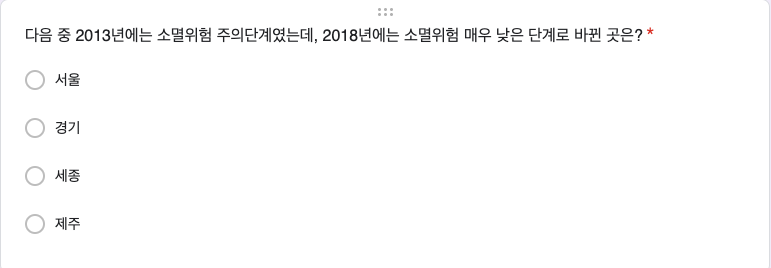
\includegraphics[width=0.75\linewidth]{./pics/Quiz230308_Q5}

\subsubsection{소멸위험 단계 개선
지역(집계표)}\label{uxc18cuxba78uxc704uxd5d8-uxb2e8uxacc4-uxac1cuxc120-uxc9c0uxc5eduxc9d1uxacc4uxd45c}

\begin{longtable}[]{@{}
  >{\raggedright\arraybackslash}p{(\columnwidth - 10\tabcolsep) * \real{0.1667}}
  >{\centering\arraybackslash}p{(\columnwidth - 10\tabcolsep) * \real{0.0972}}
  >{\centering\arraybackslash}p{(\columnwidth - 10\tabcolsep) * \real{0.0972}}
  >{\centering\arraybackslash}p{(\columnwidth - 10\tabcolsep) * \real{0.0972}}
  >{\centering\arraybackslash}p{(\columnwidth - 10\tabcolsep) * \real{0.0972}}
  >{\centering\arraybackslash}p{(\columnwidth - 10\tabcolsep) * \real{0.0972}}@{}}
\toprule\noalign{}
\begin{minipage}[b]{\linewidth}\raggedright
~
\end{minipage} & \begin{minipage}[b]{\linewidth}\centering
서울
\end{minipage} & \begin{minipage}[b]{\linewidth}\centering
경기
\end{minipage} & \begin{minipage}[b]{\linewidth}\centering
세종
\end{minipage} & \begin{minipage}[b]{\linewidth}\centering
제주
\end{minipage} & \begin{minipage}[b]{\linewidth}\centering
계
\end{minipage} \\
\midrule\noalign{}
\endhead
\bottomrule\noalign{}
\endlastfoot
\textbf{Red} & 13 & 14 & 241 & 14 & 282 \\
\textbf{Black} & 9 & 14 & 245 & 13 & 281 \\
\textbf{계} & 22 & 28 & 486 & 27 & 563 \\
\end{longtable}

\begin{longtable}[]{@{}
  >{\raggedleft\arraybackslash}p{(\columnwidth - 4\tabcolsep) * \real{0.2361}}
  >{\raggedleft\arraybackslash}p{(\columnwidth - 4\tabcolsep) * \real{0.0694}}
  >{\raggedleft\arraybackslash}p{(\columnwidth - 4\tabcolsep) * \real{0.1389}}@{}}
\caption{Pearson's Chi-squared test with simulated p-value (based on
2000 replicates): \texttt{.}}\tabularnewline
\toprule\noalign{}
\begin{minipage}[b]{\linewidth}\raggedleft
Test statistic
\end{minipage} & \begin{minipage}[b]{\linewidth}\raggedleft
df
\end{minipage} & \begin{minipage}[b]{\linewidth}\raggedleft
P value
\end{minipage} \\
\midrule\noalign{}
\endfirsthead
\toprule\noalign{}
\begin{minipage}[b]{\linewidth}\raggedleft
Test statistic
\end{minipage} & \begin{minipage}[b]{\linewidth}\raggedleft
df
\end{minipage} & \begin{minipage}[b]{\linewidth}\raggedleft
P value
\end{minipage} \\
\midrule\noalign{}
\endhead
\bottomrule\noalign{}
\endlastfoot
0.7955 & NA & 0.8721 \\
\end{longtable}

Q5의 집계 결과가 Red, Black 간에 통계적으로 유의한 차이가 있는지
알아보기 위하여 카이제곱 테스트를 수행하였습니다.

그 결과 카이제곱 통계량은 0.795, 자유도는 NA, p-value 는 0.8721이므로
Red, Black 간에 통계적으로 유의한 차이를 보이지 않습니다.

실제로 닮은 게 느껴집니까?

\subsubsection{소멸위험 단계 개선
지역(\%)}\label{uxc18cuxba78uxc704uxd5d8-uxb2e8uxacc4-uxac1cuxc120-uxc9c0uxc5ed}

\begin{longtable}[]{@{}
  >{\centering\arraybackslash}p{(\columnwidth - 8\tabcolsep) * \real{0.0972}}
  >{\centering\arraybackslash}p{(\columnwidth - 8\tabcolsep) * \real{0.0972}}
  >{\centering\arraybackslash}p{(\columnwidth - 8\tabcolsep) * \real{0.0972}}
  >{\centering\arraybackslash}p{(\columnwidth - 8\tabcolsep) * \real{0.0972}}
  >{\centering\arraybackslash}p{(\columnwidth - 8\tabcolsep) * \real{0.1111}}@{}}
\toprule\noalign{}
\begin{minipage}[b]{\linewidth}\centering
서울
\end{minipage} & \begin{minipage}[b]{\linewidth}\centering
경기
\end{minipage} & \begin{minipage}[b]{\linewidth}\centering
세종
\end{minipage} & \begin{minipage}[b]{\linewidth}\centering
제주
\end{minipage} & \begin{minipage}[b]{\linewidth}\centering
계
\end{minipage} \\
\midrule\noalign{}
\endhead
\bottomrule\noalign{}
\endlastfoot
3.9 & 5.0 & 86.3 & 4.8 & 100.0 \\
\end{longtable}

정답률은 Red, Black 을 합하여 계산하는데, 86.3(\%) 입니다.

\subsection{Q6. 조출생률과
합계출산율}\label{q6.-uxc870uxcd9cuxc0dduxb960uxacfc-uxd569uxacc4uxcd9cuxc0b0uxc728}

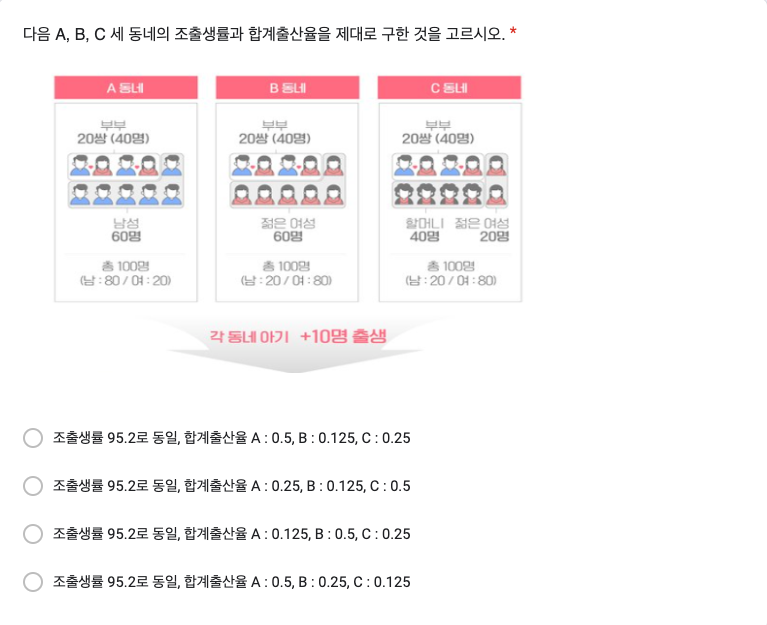
\includegraphics[width=0.75\linewidth]{./pics/Quiz230308_Q6}

\subsubsection{조출생률과
합계출산율(집계표)}\label{uxc870uxcd9cuxc0dduxb960uxacfc-uxd569uxacc4uxcd9cuxc0b0uxc728uxc9d1uxacc4uxd45c}

\begin{longtable}[]{@{}
  >{\raggedright\arraybackslash}p{(\columnwidth - 10\tabcolsep) * \real{0.0839}}
  >{\centering\arraybackslash}p{(\columnwidth - 10\tabcolsep) * \real{0.2308}}
  >{\centering\arraybackslash}p{(\columnwidth - 10\tabcolsep) * \real{0.1888}}
  >{\centering\arraybackslash}p{(\columnwidth - 10\tabcolsep) * \real{0.2308}}
  >{\centering\arraybackslash}p{(\columnwidth - 10\tabcolsep) * \real{0.2238}}
  >{\centering\arraybackslash}p{(\columnwidth - 10\tabcolsep) * \real{0.0420}}@{}}
\toprule\noalign{}
\begin{minipage}[b]{\linewidth}\raggedright
~
\end{minipage} & \begin{minipage}[b]{\linewidth}\centering
합계출산율 A : 0.5, B : 0.125, C : 0.25
\end{minipage} & \begin{minipage}[b]{\linewidth}\centering
합계출산율 A : 0.25, B : 0.125, C : 0.5
\end{minipage} & \begin{minipage}[b]{\linewidth}\centering
합계출산율 A : 0.125, B : 0.5, C : 0.25
\end{minipage} & \begin{minipage}[b]{\linewidth}\centering
합계출산율 A : 0.5, B : 0.25, C : 0.125
\end{minipage} & \begin{minipage}[b]{\linewidth}\centering
계
\end{minipage} \\
\midrule\noalign{}
\endhead
\bottomrule\noalign{}
\endlastfoot
\textbf{Red} & 163 & 34 & 56 & 29 & 282 \\
\textbf{Black} & 140 & 56 & 48 & 37 & 281 \\
\textbf{계} & 303 & 90 & 104 & 66 & 563 \\
\end{longtable}

\begin{longtable}[]{@{}
  >{\raggedleft\arraybackslash}p{(\columnwidth - 4\tabcolsep) * \real{0.2361}}
  >{\raggedleft\arraybackslash}p{(\columnwidth - 4\tabcolsep) * \real{0.0694}}
  >{\raggedleft\arraybackslash}p{(\columnwidth - 4\tabcolsep) * \real{0.1667}}@{}}
\caption{Pearson's Chi-squared test: \texttt{.}}\tabularnewline
\toprule\noalign{}
\begin{minipage}[b]{\linewidth}\raggedleft
Test statistic
\end{minipage} & \begin{minipage}[b]{\linewidth}\raggedleft
df
\end{minipage} & \begin{minipage}[b]{\linewidth}\raggedleft
P value
\end{minipage} \\
\midrule\noalign{}
\endfirsthead
\toprule\noalign{}
\begin{minipage}[b]{\linewidth}\raggedleft
Test statistic
\end{minipage} & \begin{minipage}[b]{\linewidth}\raggedleft
df
\end{minipage} & \begin{minipage}[b]{\linewidth}\raggedleft
P value
\end{minipage} \\
\midrule\noalign{}
\endhead
\bottomrule\noalign{}
\endlastfoot
8.707 & 3 & 0.03345 * \\
\end{longtable}

Q6의 집계 결과가 Red, Black 간에 통계적으로 유의한 차이가 있는지
알아보기 위하여 카이제곱 테스트를 수행하였습니다.

그 결과 카이제곱 통계량은 8.707, 자유도는 3, p-value 는 0.0335이므로
Red, Black 간에 통계적으로 유의한 차이를 보이고 있습니다.

\subsubsection{조출생률과
합계출산율(\%)}\label{uxc870uxcd9cuxc0dduxb960uxacfc-uxd569uxacc4uxcd9cuxc0b0uxc728}

\begin{longtable}[]{@{}
  >{\centering\arraybackslash}p{(\columnwidth - 8\tabcolsep) * \real{0.2481}}
  >{\centering\arraybackslash}p{(\columnwidth - 8\tabcolsep) * \real{0.2030}}
  >{\centering\arraybackslash}p{(\columnwidth - 8\tabcolsep) * \real{0.2481}}
  >{\centering\arraybackslash}p{(\columnwidth - 8\tabcolsep) * \real{0.2406}}
  >{\centering\arraybackslash}p{(\columnwidth - 8\tabcolsep) * \real{0.0602}}@{}}
\toprule\noalign{}
\begin{minipage}[b]{\linewidth}\centering
합계출산율 A : 0.5, B : 0.125, C : 0.25
\end{minipage} & \begin{minipage}[b]{\linewidth}\centering
합계출산율 A : 0.25, B : 0.125, C : 0.5
\end{minipage} & \begin{minipage}[b]{\linewidth}\centering
합계출산율 A : 0.125, B : 0.5, C : 0.25
\end{minipage} & \begin{minipage}[b]{\linewidth}\centering
합계출산율 A : 0.5, B : 0.25, C : 0.125
\end{minipage} & \begin{minipage}[b]{\linewidth}\centering
계
\end{minipage} \\
\midrule\noalign{}
\endhead
\bottomrule\noalign{}
\endlastfoot
53.8 & 16.0 & 18.5 & 11.7 & 100.0 \\
\end{longtable}

정답률은 Red, Black 을 합하여 계산하는데, 53.8(\%) 입니다.

\subsection{Q7. 눈속임 그래프(Cheating
Charts)}\label{q7.-uxb208uxc18duxc784-uxadf8uxb798uxd504cheating-charts}

지난 학기까지 앞에 나오는 선지를 고르기 쉽다는 1번효과에 대한 질문을
만들어서 테스트해 왔지만 효과를 검증하기 어려워 문제를 바꿔 보았습니다.

언론방송에서 가끔 원형그래프나 막대그래프를 제시하면서 숫자와 그림이
맞지 않는 경우를 볼 수 있습니다.

여러분들은 그런 경우에 어떻게 인식하는 지 언론기관에서 발표한 눈속임
그래프를 보여줍니다.

Red에는 원형그래프의 각도를 속이고, Black 에는 막대그래프의 높이를 속여
어떤 응답이 나오는 지 살펴보았습니다.

여러분들은 대부분 눈속임 그래프에 속지 않고 있습니다.

언론기관들이 왜 이런 짓들을 하는지 궁금해집니다.

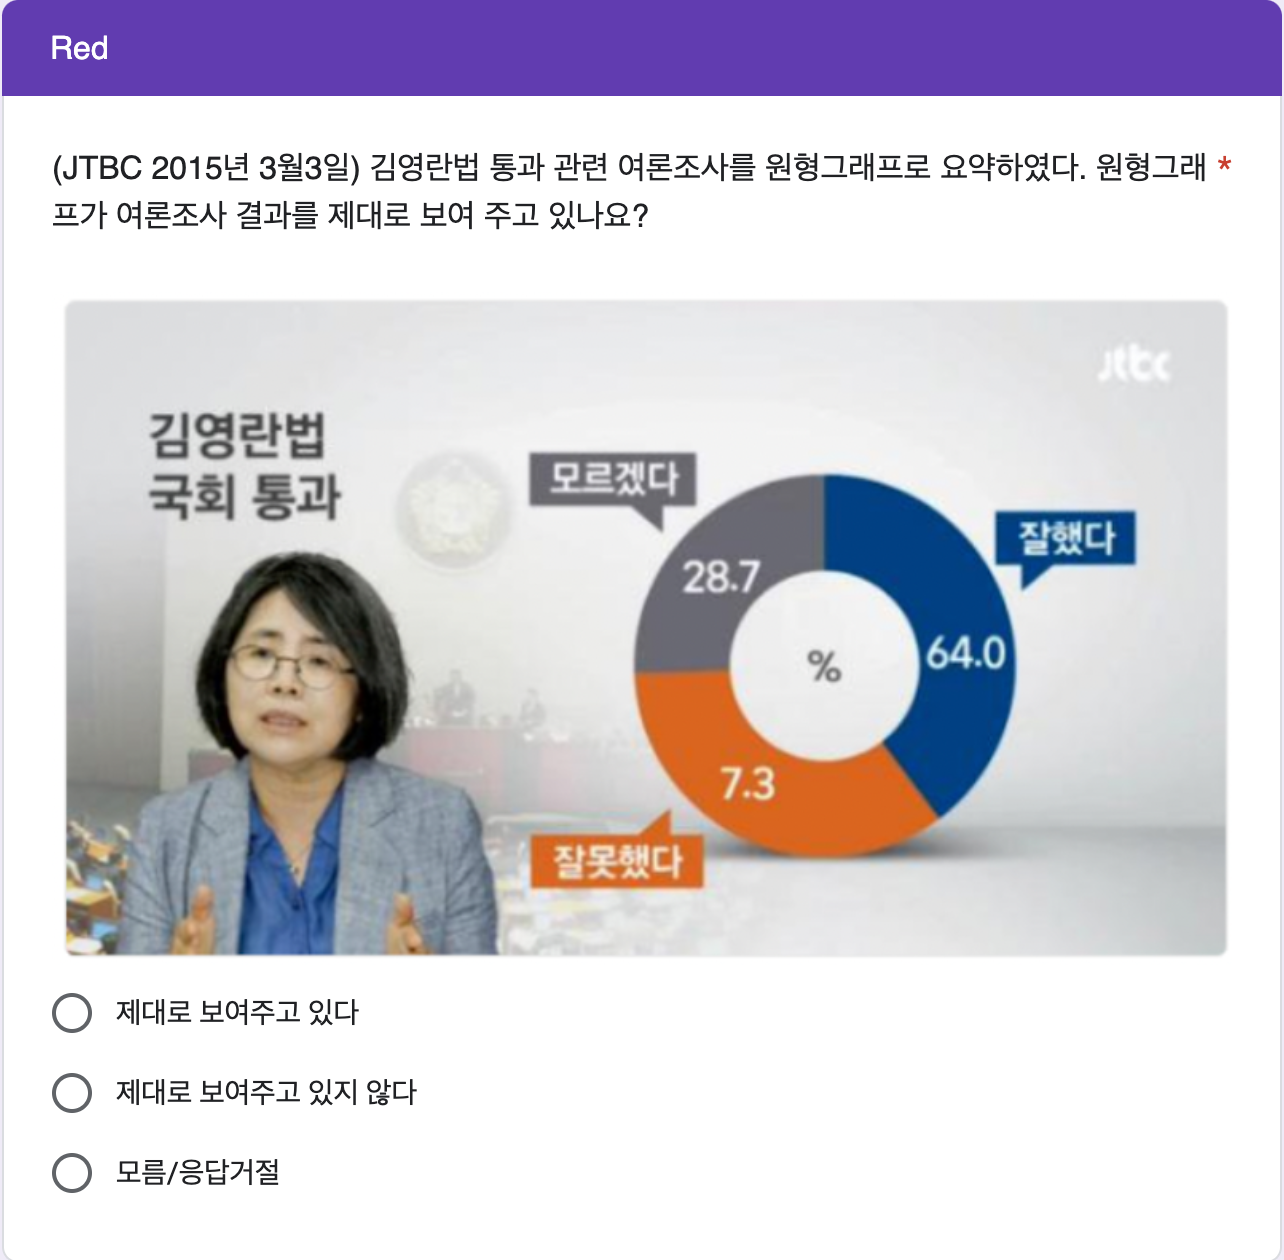
\includegraphics[width=0.67\linewidth]{./pics/Quiz240308_Q7_Red}

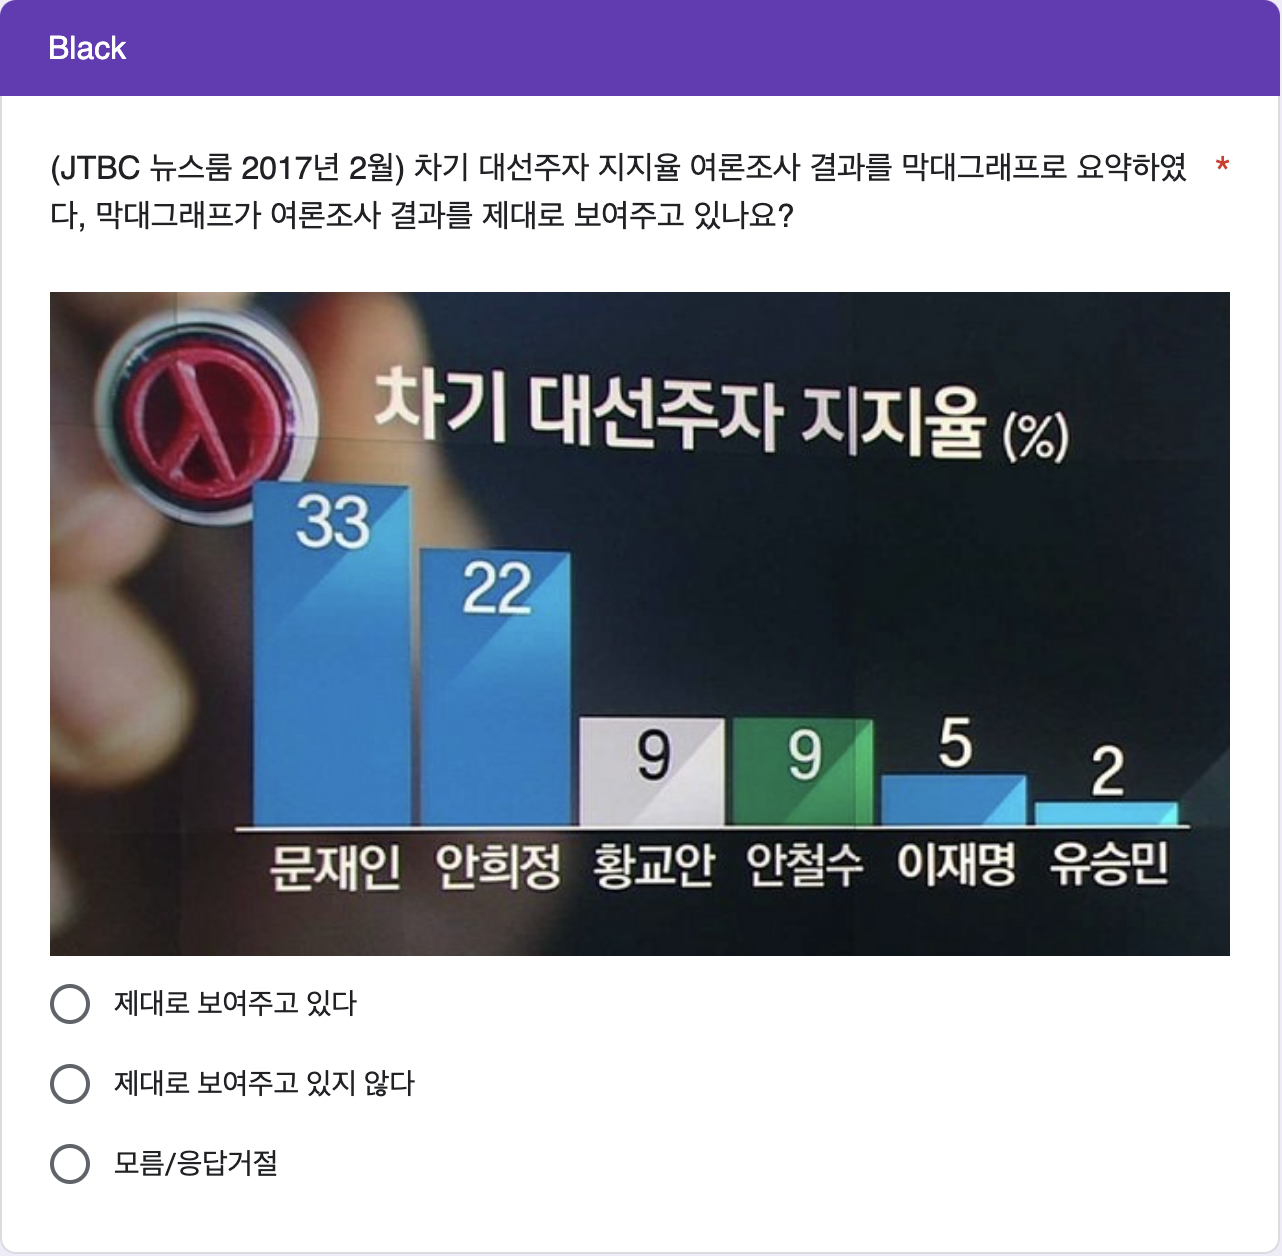
\includegraphics[width=0.67\linewidth]{./pics/Quiz240308_Q7_Black}

\subsubsection{집계표}\label{uxc9d1uxacc4uxd45c}

\begin{longtable}[]{@{}
  >{\raggedright\arraybackslash}p{(\columnwidth - 8\tabcolsep) * \real{0.3048}}
  >{\centering\arraybackslash}p{(\columnwidth - 8\tabcolsep) * \real{0.2190}}
  >{\centering\arraybackslash}p{(\columnwidth - 8\tabcolsep) * \real{0.2667}}
  >{\centering\arraybackslash}p{(\columnwidth - 8\tabcolsep) * \real{0.1524}}
  >{\centering\arraybackslash}p{(\columnwidth - 8\tabcolsep) * \real{0.0571}}@{}}
\toprule\noalign{}
\begin{minipage}[b]{\linewidth}\raggedright
~
\end{minipage} & \begin{minipage}[b]{\linewidth}\centering
제대로 보여주고 있다
\end{minipage} & \begin{minipage}[b]{\linewidth}\centering
제대로 보여주고 있지 않다
\end{minipage} & \begin{minipage}[b]{\linewidth}\centering
모름/응답거절
\end{minipage} & \begin{minipage}[b]{\linewidth}\centering
계
\end{minipage} \\
\midrule\noalign{}
\endhead
\bottomrule\noalign{}
\endlastfoot
\textbf{Red(김영란법 국회통과)} & 65 & 180 & 37 & 282 \\
\textbf{Black(고위공직자 범죄수사처 설립)} & 100 & 119 & 62 & 281 \\
\textbf{계} & 165 & 299 & 99 & 563 \\
\end{longtable}

\begin{longtable}[]{@{}
  >{\raggedleft\arraybackslash}p{(\columnwidth - 4\tabcolsep) * \real{0.2361}}
  >{\raggedleft\arraybackslash}p{(\columnwidth - 4\tabcolsep) * \real{0.0694}}
  >{\raggedleft\arraybackslash}p{(\columnwidth - 4\tabcolsep) * \real{0.2500}}@{}}
\caption{Pearson's Chi-squared test: \texttt{.}}\tabularnewline
\toprule\noalign{}
\begin{minipage}[b]{\linewidth}\raggedleft
Test statistic
\end{minipage} & \begin{minipage}[b]{\linewidth}\raggedleft
df
\end{minipage} & \begin{minipage}[b]{\linewidth}\raggedleft
P value
\end{minipage} \\
\midrule\noalign{}
\endfirsthead
\toprule\noalign{}
\begin{minipage}[b]{\linewidth}\raggedleft
Test statistic
\end{minipage} & \begin{minipage}[b]{\linewidth}\raggedleft
df
\end{minipage} & \begin{minipage}[b]{\linewidth}\raggedleft
P value
\end{minipage} \\
\midrule\noalign{}
\endhead
\bottomrule\noalign{}
\endlastfoot
26.18 & 2 & 2.065e-06 * * * \\
\end{longtable}

Q7의 Red에는 김영란법 국회통과에 대한 여론조사 결과를 원형그래프로
나타내었는데 잘했다(64\%), 잘못했다(7.3\%), 모르겠다(28.7\%)의 각도를
데이터와 전혀 맞지 않게 왜곡하여 마치 잘했다와 잘못했다의 비율이 거의
대등한 것처럼 각도를 조정하였습니다.

282명이 응답한 가운데 65명이 결과를 ``제대로 보여주고 있다''는 반응을
보이고, 180명이 결과를 ``제대로 보여주고 있지 않다''는 반응을 보입니다.

Black은 2017년 대선의 대선주자 여론조사에서 33\%의 지지율을 기록한
문재인 예비후보와 22\%의 지지율을 기록한 안희정 예비후보의 지지율 막대가
거의 비슷한 것처럼 왜곡하였습니다.

281명이 응답한 가운데 100명이 여론조사 결과를 '' 제대로 보여주고
있다''는 반응을 보이고, 119명이 여론조사 결과를 ``제대로 보여주고 있지
않다''는 반응을 보입니다.

그리고 ``모름/무응답''에 답한 인원은 Red에 37명, Black 에 62명이
었습니다.

카이제곱 테스트는 이와 같은 상황에서 원형그래프를 왜곡할 떄와
막대그래프를 왜곡할 때 인식의 차이가 통계적으로 유의하다는 것을 보여
줍니다.

카이제곱 통계량은 26.180, 자유도는 2, p-value 는 2.1e-06(으)로 그래프의
유형에 따라 눈속임의 인식에 통계적으로 유의한 차이가 관찰된다는 것을
보여줍니다.

여기서 그래프의 유형이 눈속임의 인식에 차이를 주지 않는다고 가정합니다.

랜덤화의 효과로 Red, Black 의 응답은 닮게 마련입니다.

즉, 통계적으로 유의한 차이를 보이지 않게 됩니다.

그러나 실제로 관찰된 카이제곱 통계값의 P-value 는 0.05보다 매우 작은
값입니다.

따라서, 그래프의 유형이 눈속임의 인식에 영향을 끼치지 않는다는 가정은
잘못된 것이죠.

이러한 논증 방식을 귀류법이라고 합니다.

\subsubsection{\% 비교}\label{uxbe44uxad50}

\begin{longtable}[]{@{}
  >{\raggedright\arraybackslash}p{(\columnwidth - 8\tabcolsep) * \real{0.2991}}
  >{\centering\arraybackslash}p{(\columnwidth - 8\tabcolsep) * \real{0.2150}}
  >{\centering\arraybackslash}p{(\columnwidth - 8\tabcolsep) * \real{0.2617}}
  >{\centering\arraybackslash}p{(\columnwidth - 8\tabcolsep) * \real{0.1495}}
  >{\centering\arraybackslash}p{(\columnwidth - 8\tabcolsep) * \real{0.0748}}@{}}
\toprule\noalign{}
\begin{minipage}[b]{\linewidth}\raggedright
~
\end{minipage} & \begin{minipage}[b]{\linewidth}\centering
제대로 보여주고 있다
\end{minipage} & \begin{minipage}[b]{\linewidth}\centering
제대로 보여주고 있지 않다
\end{minipage} & \begin{minipage}[b]{\linewidth}\centering
모름/응답거절
\end{minipage} & \begin{minipage}[b]{\linewidth}\centering
계
\end{minipage} \\
\midrule\noalign{}
\endhead
\bottomrule\noalign{}
\endlastfoot
\textbf{Red(김영란법 국회통과)} & 23.0 & 63.8 & 13.1 & 100.0 \\
\textbf{Black(고위공직자 범죄수사처 설립)} & 35.6 & 42.3 & 22.1 &
100.0 \\
\end{longtable}

원형그래프의 각도를 왜곡한 Red에서 여론조사 결과를 ``제대로 보여주고
있다''고 응답하는 사람들의 백분율, 23.0(\%)은 ``제대로 보여주고 있지
않다''고 응답하는 사람들의 백분율, 63.8(\%) 보다 매우 낮습니다.

반면 막대그래프의 높이를 왜곡한 Black에서 여론조사 결과를 ``제대로
보여주고 있다''고 응답하는 사람들의 백분율, 35.6(\%)은 ``제대로 보여주고
있지 않다''고 응답하는 사람들의 백분율, 42.3(\%) 보다 적습니다.

원형그래프에서 눈속임을 지각하는 백분율이 막대그래프에서 눈속임을
지각하는 백분율보다 훨씬 높게 나타나고 있습니다.

원형그래프의 각도를 속이느냐, 막대그래프의 높이를 속이느냐에 따라 반응이
달라진다는 것을 잘 알 수 있습니다.

\subsubsection{Mosaic Plot}\label{mosaic-plot}


\includegraphics{quiz250310_Report_v6_files/figure-latex/mosaic plot-1.pdf}

Mosaic Plot 은 이 집계결과를 시각적으로 잘 보여줍니다.

원형그래프의 각도를 왜곡한 Red 에서 여론조사 결과를 ``제대로 보여주고
있다''고 응답한 백분율이 매우 낮고, 막대그래프의 높이를 왜곡한 Black
에서 여론조사 결과를 ``제대로 보여주고 있다''고 응답한 백분율은
상대적으로 덜 낮은 것을 시각적으로 알 수 있습니다.

\subsection{마감 시간으로부터 제출 시간의
분포}\label{uxb9c8uxac10-uxc2dcuxac04uxc73cuxb85cuxbd80uxd130-uxc81cuxcd9c-uxc2dcuxac04uxc758-uxbd84uxd3ec}

\subsubsection{분포표}\label{uxbd84uxd3ecuxd45c}

\begin{longtable}[]{@{}
  >{\raggedright\arraybackslash}p{(\columnwidth - 30\tabcolsep) * \real{0.0863}}
  >{\raggedleft\arraybackslash}p{(\columnwidth - 30\tabcolsep) * \real{0.0576}}
  >{\raggedleft\arraybackslash}p{(\columnwidth - 30\tabcolsep) * \real{0.0576}}
  >{\raggedleft\arraybackslash}p{(\columnwidth - 30\tabcolsep) * \real{0.0576}}
  >{\raggedleft\arraybackslash}p{(\columnwidth - 30\tabcolsep) * \real{0.0576}}
  >{\raggedleft\arraybackslash}p{(\columnwidth - 30\tabcolsep) * \real{0.0576}}
  >{\raggedleft\arraybackslash}p{(\columnwidth - 30\tabcolsep) * \real{0.0576}}
  >{\raggedleft\arraybackslash}p{(\columnwidth - 30\tabcolsep) * \real{0.0576}}
  >{\raggedleft\arraybackslash}p{(\columnwidth - 30\tabcolsep) * \real{0.0576}}
  >{\raggedleft\arraybackslash}p{(\columnwidth - 30\tabcolsep) * \real{0.0576}}
  >{\raggedleft\arraybackslash}p{(\columnwidth - 30\tabcolsep) * \real{0.0647}}
  >{\raggedleft\arraybackslash}p{(\columnwidth - 30\tabcolsep) * \real{0.0719}}
  >{\raggedleft\arraybackslash}p{(\columnwidth - 30\tabcolsep) * \real{0.0719}}
  >{\raggedleft\arraybackslash}p{(\columnwidth - 30\tabcolsep) * \real{0.0719}}
  >{\raggedleft\arraybackslash}p{(\columnwidth - 30\tabcolsep) * \real{0.0719}}
  >{\centering\arraybackslash}p{(\columnwidth - 30\tabcolsep) * \real{0.0432}}@{}}
\caption{일 단위}\tabularnewline
\toprule\noalign{}
\begin{minipage}[b]{\linewidth}\raggedright
~
\end{minipage} & \begin{minipage}[b]{\linewidth}\raggedleft
{[}0,1{]}
\end{minipage} & \begin{minipage}[b]{\linewidth}\raggedleft
(1,2{]}
\end{minipage} & \begin{minipage}[b]{\linewidth}\raggedleft
(2,3{]}
\end{minipage} & \begin{minipage}[b]{\linewidth}\raggedleft
(3,4{]}
\end{minipage} & \begin{minipage}[b]{\linewidth}\raggedleft
(4,5{]}
\end{minipage} & \begin{minipage}[b]{\linewidth}\raggedleft
(5,6{]}
\end{minipage} & \begin{minipage}[b]{\linewidth}\raggedleft
(6,7{]}
\end{minipage} & \begin{minipage}[b]{\linewidth}\raggedleft
(7,8{]}
\end{minipage} & \begin{minipage}[b]{\linewidth}\raggedleft
(8,9{]}
\end{minipage} & \begin{minipage}[b]{\linewidth}\raggedleft
(9,10{]}
\end{minipage} & \begin{minipage}[b]{\linewidth}\raggedleft
(10,11{]}
\end{minipage} & \begin{minipage}[b]{\linewidth}\raggedleft
(11,12{]}
\end{minipage} & \begin{minipage}[b]{\linewidth}\raggedleft
(12,13{]}
\end{minipage} & \begin{minipage}[b]{\linewidth}\raggedleft
(13,14{]}
\end{minipage} & \begin{minipage}[b]{\linewidth}\centering
계
\end{minipage} \\
\midrule\noalign{}
\endfirsthead
\toprule\noalign{}
\begin{minipage}[b]{\linewidth}\raggedright
~
\end{minipage} & \begin{minipage}[b]{\linewidth}\raggedleft
{[}0,1{]}
\end{minipage} & \begin{minipage}[b]{\linewidth}\raggedleft
(1,2{]}
\end{minipage} & \begin{minipage}[b]{\linewidth}\raggedleft
(2,3{]}
\end{minipage} & \begin{minipage}[b]{\linewidth}\raggedleft
(3,4{]}
\end{minipage} & \begin{minipage}[b]{\linewidth}\raggedleft
(4,5{]}
\end{minipage} & \begin{minipage}[b]{\linewidth}\raggedleft
(5,6{]}
\end{minipage} & \begin{minipage}[b]{\linewidth}\raggedleft
(6,7{]}
\end{minipage} & \begin{minipage}[b]{\linewidth}\raggedleft
(7,8{]}
\end{minipage} & \begin{minipage}[b]{\linewidth}\raggedleft
(8,9{]}
\end{minipage} & \begin{minipage}[b]{\linewidth}\raggedleft
(9,10{]}
\end{minipage} & \begin{minipage}[b]{\linewidth}\raggedleft
(10,11{]}
\end{minipage} & \begin{minipage}[b]{\linewidth}\raggedleft
(11,12{]}
\end{minipage} & \begin{minipage}[b]{\linewidth}\raggedleft
(12,13{]}
\end{minipage} & \begin{minipage}[b]{\linewidth}\raggedleft
(13,14{]}
\end{minipage} & \begin{minipage}[b]{\linewidth}\centering
계
\end{minipage} \\
\midrule\noalign{}
\endhead
\bottomrule\noalign{}
\endlastfoot
\textbf{Red} & 52 & 17 & 9 & 6 & 12 & 8 & 12 & 51 & 20 & 13 & 21 & 13 &
21 & 27 & 282 \\
\textbf{Black} & 59 & 11 & 11 & 3 & 6 & 7 & 9 & 43 & 19 & 18 & 20 & 21 &
26 & 28 & 281 \\
\textbf{계} & 111 & 28 & 20 & 9 & 18 & 15 & 21 & 94 & 39 & 31 & 41 & 34
& 47 & 55 & 563 \\
\end{longtable}

분포표로부터 두 가지 문제를 살펴보겠습니다.

첫째, 날마다 고르게 제출하는가?

둘쨰, Red, Black 간에 통계적으로 유의한 차이가 있는가?

각 문제를 살펴보기 위해서는 분포표의 일부분을 대상으로 카이제곱 테스트를
수행합니다.

\subsubsection{날마다 고르게
제출하는가?}\label{uxb0a0uxb9c8uxb2e4-uxace0uxb974uxac8c-uxc81cuxcd9cuxd558uxb294uxac00}

\begin{longtable}[]{@{}
  >{\raggedleft\arraybackslash}p{(\columnwidth - 24\tabcolsep) * \real{0.0708}}
  >{\raggedleft\arraybackslash}p{(\columnwidth - 24\tabcolsep) * \real{0.0708}}
  >{\raggedleft\arraybackslash}p{(\columnwidth - 24\tabcolsep) * \real{0.0708}}
  >{\raggedleft\arraybackslash}p{(\columnwidth - 24\tabcolsep) * \real{0.0708}}
  >{\raggedleft\arraybackslash}p{(\columnwidth - 24\tabcolsep) * \real{0.0708}}
  >{\raggedleft\arraybackslash}p{(\columnwidth - 24\tabcolsep) * \real{0.0708}}
  >{\raggedleft\arraybackslash}p{(\columnwidth - 24\tabcolsep) * \real{0.0708}}
  >{\raggedleft\arraybackslash}p{(\columnwidth - 24\tabcolsep) * \real{0.0708}}
  >{\raggedleft\arraybackslash}p{(\columnwidth - 24\tabcolsep) * \real{0.0796}}
  >{\raggedleft\arraybackslash}p{(\columnwidth - 24\tabcolsep) * \real{0.0885}}
  >{\raggedleft\arraybackslash}p{(\columnwidth - 24\tabcolsep) * \real{0.0885}}
  >{\raggedleft\arraybackslash}p{(\columnwidth - 24\tabcolsep) * \real{0.0885}}
  >{\raggedleft\arraybackslash}p{(\columnwidth - 24\tabcolsep) * \real{0.0885}}@{}}
\toprule\noalign{}
\begin{minipage}[b]{\linewidth}\raggedleft
(1,2{]}
\end{minipage} & \begin{minipage}[b]{\linewidth}\raggedleft
(2,3{]}
\end{minipage} & \begin{minipage}[b]{\linewidth}\raggedleft
(3,4{]}
\end{minipage} & \begin{minipage}[b]{\linewidth}\raggedleft
(4,5{]}
\end{minipage} & \begin{minipage}[b]{\linewidth}\raggedleft
(5,6{]}
\end{minipage} & \begin{minipage}[b]{\linewidth}\raggedleft
(6,7{]}
\end{minipage} & \begin{minipage}[b]{\linewidth}\raggedleft
(7,8{]}
\end{minipage} & \begin{minipage}[b]{\linewidth}\raggedleft
(8,9{]}
\end{minipage} & \begin{minipage}[b]{\linewidth}\raggedleft
(9,10{]}
\end{minipage} & \begin{minipage}[b]{\linewidth}\raggedleft
(10,11{]}
\end{minipage} & \begin{minipage}[b]{\linewidth}\raggedleft
(11,12{]}
\end{minipage} & \begin{minipage}[b]{\linewidth}\raggedleft
(12,13{]}
\end{minipage} & \begin{minipage}[b]{\linewidth}\raggedleft
(13,14{]}
\end{minipage} \\
\midrule\noalign{}
\endhead
\bottomrule\noalign{}
\endlastfoot
28 & 20 & 9 & 18 & 15 & 21 & 94 & 39 & 31 & 41 & 34 & 47 & 55 \\
\end{longtable}

\begin{longtable}[]{@{}
  >{\raggedleft\arraybackslash}p{(\columnwidth - 4\tabcolsep) * \real{0.2361}}
  >{\raggedleft\arraybackslash}p{(\columnwidth - 4\tabcolsep) * \real{0.0694}}
  >{\raggedleft\arraybackslash}p{(\columnwidth - 4\tabcolsep) * \real{0.2500}}@{}}
\caption{Chi-squared test for given probabilities:
\texttt{.}}\tabularnewline
\toprule\noalign{}
\begin{minipage}[b]{\linewidth}\raggedleft
Test statistic
\end{minipage} & \begin{minipage}[b]{\linewidth}\raggedleft
df
\end{minipage} & \begin{minipage}[b]{\linewidth}\raggedleft
P value
\end{minipage} \\
\midrule\noalign{}
\endfirsthead
\toprule\noalign{}
\begin{minipage}[b]{\linewidth}\raggedleft
Test statistic
\end{minipage} & \begin{minipage}[b]{\linewidth}\raggedleft
df
\end{minipage} & \begin{minipage}[b]{\linewidth}\raggedleft
P value
\end{minipage} \\
\midrule\noalign{}
\endhead
\bottomrule\noalign{}
\endlastfoot
170.5 & 12 & 3.764e-30 * * * \\
\end{longtable}

날마다 고르게 제출하는지 알아 보았습니다.

분포표의 ``계''행에서 '계'열을 제외하고 카이제곱테스트를 수행합니다.

분포표 만으로도 쉽게 파악할 수 있지만 카이제곱테스트가 명확히 해 줍니다.

카이제곱 통계량은 170.50, 자유도는 12.00, p-value 는 3.8e-30 이므로 결코
고르게 제출한다고 말할 수 없겠습니다.

막대그래프로 살펴 보겠습니다.

\subsubsection{막대그래프}\label{uxb9c9uxb300uxadf8uxb798uxd504}

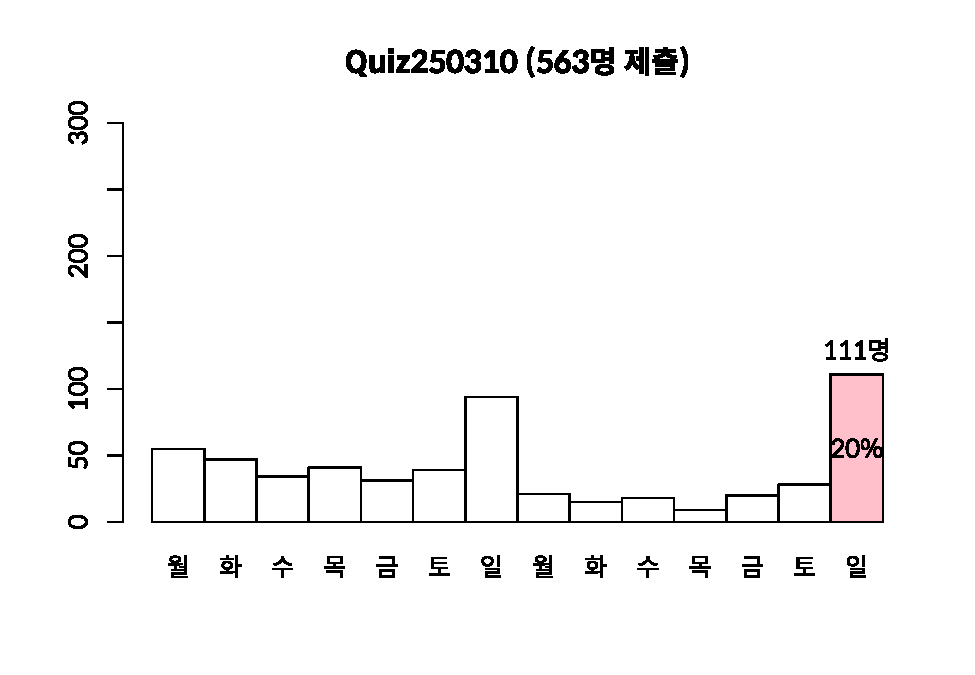
\includegraphics{quiz250310_Report_v6_files/figure-latex/unnamed-chunk-15-1.pdf}

막대그래프는 총 제출인원 563(명) 중에 111(명), 20(\%)가 마감일에 몰리는
것을 명확히 보여주고 있습니다.

\subsubsection{Red, Black 간에
닮았는가?}\label{red-black-uxac04uxc5d0-uxb2eeuxc558uxb294uxac00}

\begin{longtable}[]{@{}
  >{\raggedright\arraybackslash}p{(\columnwidth - 26\tabcolsep) * \real{0.0960}}
  >{\raggedleft\arraybackslash}p{(\columnwidth - 26\tabcolsep) * \real{0.0640}}
  >{\raggedleft\arraybackslash}p{(\columnwidth - 26\tabcolsep) * \real{0.0640}}
  >{\raggedleft\arraybackslash}p{(\columnwidth - 26\tabcolsep) * \real{0.0640}}
  >{\raggedleft\arraybackslash}p{(\columnwidth - 26\tabcolsep) * \real{0.0640}}
  >{\raggedleft\arraybackslash}p{(\columnwidth - 26\tabcolsep) * \real{0.0640}}
  >{\raggedleft\arraybackslash}p{(\columnwidth - 26\tabcolsep) * \real{0.0640}}
  >{\raggedleft\arraybackslash}p{(\columnwidth - 26\tabcolsep) * \real{0.0640}}
  >{\raggedleft\arraybackslash}p{(\columnwidth - 26\tabcolsep) * \real{0.0640}}
  >{\raggedleft\arraybackslash}p{(\columnwidth - 26\tabcolsep) * \real{0.0720}}
  >{\raggedleft\arraybackslash}p{(\columnwidth - 26\tabcolsep) * \real{0.0800}}
  >{\raggedleft\arraybackslash}p{(\columnwidth - 26\tabcolsep) * \real{0.0800}}
  >{\raggedleft\arraybackslash}p{(\columnwidth - 26\tabcolsep) * \real{0.0800}}
  >{\raggedleft\arraybackslash}p{(\columnwidth - 26\tabcolsep) * \real{0.0800}}@{}}
\toprule\noalign{}
\begin{minipage}[b]{\linewidth}\raggedright
~
\end{minipage} & \begin{minipage}[b]{\linewidth}\raggedleft
(1,2{]}
\end{minipage} & \begin{minipage}[b]{\linewidth}\raggedleft
(2,3{]}
\end{minipage} & \begin{minipage}[b]{\linewidth}\raggedleft
(3,4{]}
\end{minipage} & \begin{minipage}[b]{\linewidth}\raggedleft
(4,5{]}
\end{minipage} & \begin{minipage}[b]{\linewidth}\raggedleft
(5,6{]}
\end{minipage} & \begin{minipage}[b]{\linewidth}\raggedleft
(6,7{]}
\end{minipage} & \begin{minipage}[b]{\linewidth}\raggedleft
(7,8{]}
\end{minipage} & \begin{minipage}[b]{\linewidth}\raggedleft
(8,9{]}
\end{minipage} & \begin{minipage}[b]{\linewidth}\raggedleft
(9,10{]}
\end{minipage} & \begin{minipage}[b]{\linewidth}\raggedleft
(10,11{]}
\end{minipage} & \begin{minipage}[b]{\linewidth}\raggedleft
(11,12{]}
\end{minipage} & \begin{minipage}[b]{\linewidth}\raggedleft
(12,13{]}
\end{minipage} & \begin{minipage}[b]{\linewidth}\raggedleft
(13,14{]}
\end{minipage} \\
\midrule\noalign{}
\endhead
\bottomrule\noalign{}
\endlastfoot
\textbf{Red} & 17 & 9 & 6 & 12 & 8 & 12 & 51 & 20 & 13 & 21 & 13 & 21 &
27 \\
\textbf{Black} & 11 & 11 & 3 & 6 & 7 & 9 & 43 & 19 & 18 & 20 & 21 & 26 &
28 \\
\end{longtable}

\begin{longtable}[]{@{}
  >{\raggedleft\arraybackslash}p{(\columnwidth - 4\tabcolsep) * \real{0.2361}}
  >{\raggedleft\arraybackslash}p{(\columnwidth - 4\tabcolsep) * \real{0.0694}}
  >{\raggedleft\arraybackslash}p{(\columnwidth - 4\tabcolsep) * \real{0.1389}}@{}}
\caption{Pearson's Chi-squared test: \texttt{.}}\tabularnewline
\toprule\noalign{}
\begin{minipage}[b]{\linewidth}\raggedleft
Test statistic
\end{minipage} & \begin{minipage}[b]{\linewidth}\raggedleft
df
\end{minipage} & \begin{minipage}[b]{\linewidth}\raggedleft
P value
\end{minipage} \\
\midrule\noalign{}
\endfirsthead
\toprule\noalign{}
\begin{minipage}[b]{\linewidth}\raggedleft
Test statistic
\end{minipage} & \begin{minipage}[b]{\linewidth}\raggedleft
df
\end{minipage} & \begin{minipage}[b]{\linewidth}\raggedleft
P value
\end{minipage} \\
\midrule\noalign{}
\endhead
\bottomrule\noalign{}
\endlastfoot
8.812 & 12 & 0.7189 \\
\end{longtable}

제출시간의 분포가 Red, Black 간에 닮았는지 알아 보았습니다.

이번에는 분포표의 첫번째와 두번째 행, '계'열을 제외한 나머지 열에 대해서
카이제곱테스트를 수행합니다.

카이제곱 통계량은 8.812, 자유도는 12, p-value 는 0.7189 이므로 제출
시간의 분포는 Red, Black 간에 통계적으로 유의한 차이가 관찰되지
않습니다.

이 사실을 Mosaic Plot 을 이용하여 시각적으로 살펴보겠습니다.

닮았다고 느껴지나요?

\subsubsection{Mosaic Plot}\label{mosaic-plot-1}

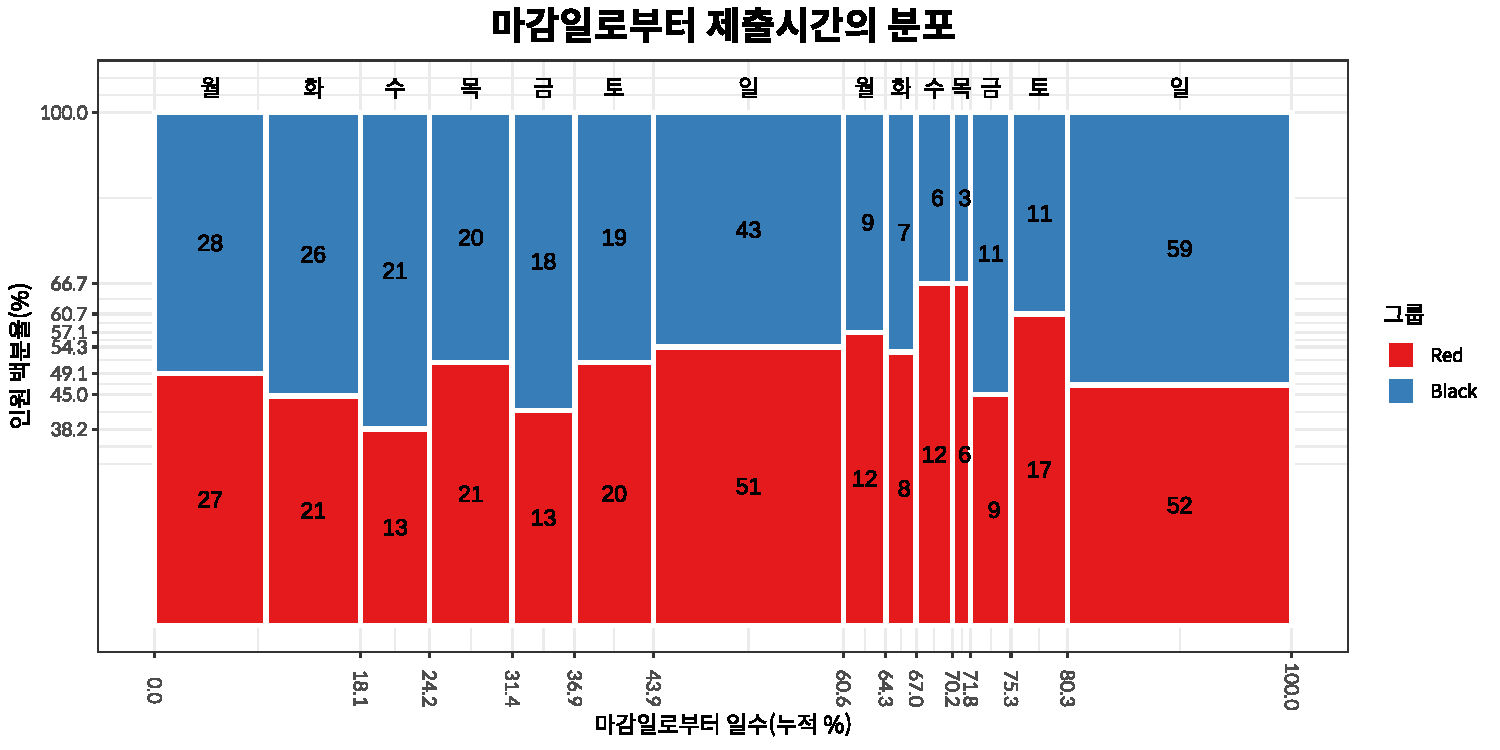
\includegraphics{quiz250310_Report_v6_files/figure-latex/unnamed-chunk-17-1.pdf}

\end{document}
